
\chapter{Implementation of an Installable Client Driver for Altera OpenCL}
\label{section:icd}

As of SDK version 13.1 (which is used in this thesis) all Altera OpenCL functions are implemented in the dynamic library \texttt{libalteracl.so}.
Using this library directly inhibits the use of a second OpenCL implementation from a different vendor in the same application.
Trying to link both libraries during compilation will fail due to conflicting multiple symbol definitions.

The \texttt{cl\_khr\_icd} OpenCL extension \cite{icd} defines the \emph{Installable Client Driver} (ICD) and the \emph{ICD Loader} libraries that act as a proxy between the user program and the actual implementations.
With this extension, the vendor implementations are loaded at run time, avoiding the issue of symbol conflicts.
The application is then linked to the ICD Loader instead of the individual vendor libraries.
Figure \ref{fig:icd} illustrates the relationships between the libraries.
Currently, Altera does not provide an ICD for its SDK.
A minimal ICD was implemented during this thesis and it is documented in this section.


%NVIDIA ICD is called libnvidia-opencl.so.1 and dlopens (most likely) libcuda.so
\begin{figure}[htb]
\centerline{
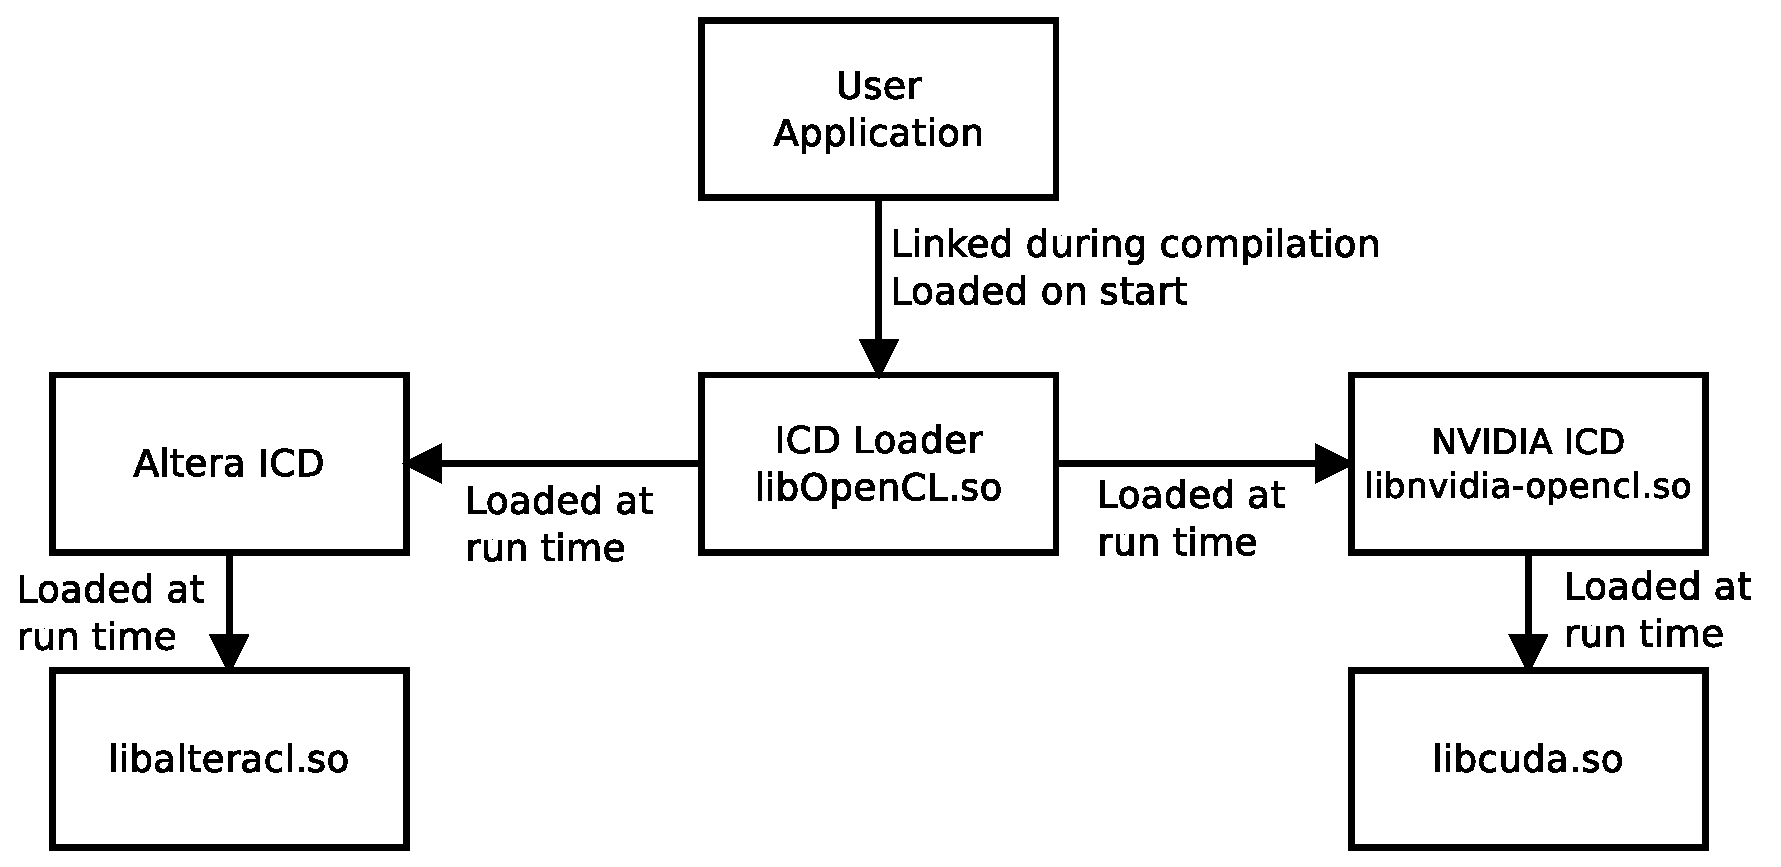
\includegraphics[width=0.85\textwidth]{images/icd.eps}}
\caption{Relationship between the dynamic libraries}
\label{fig:icd}
\end{figure}


%extension specs

To enumerate vendor ICDs on Linux, the ICD Loader scans the files located in the path \texttt{/etc/OpenCL/vendors} \cite{icd}.
These files have to contain a single line with the absolute or relative path to the actual vendor ICD dynamic library.
The loader will then attempt to load this library using \texttt{dlopen}.
%If successful, the functions \texttt{clIcdGetPlatformIDsKHR}, \texttt{clGetPlatformInfo}, and \texttt{clGetExtensionFunctionAddress} are queried.

The extension re-defines all OpenCL functions and objects.
When the user application calls an OpenCL function it actually calls one of those re-defined functions from the ICD Loader.
The first function, of an OpenCL application is usually \texttt{clGetPlatformIDs}.
When it is called, the ICD Loader iterates over all known vendor ICDs and in turn calls their \texttt{clGetPlatformIDs}.
The vendor ICD then returns a pointer to a struct which has to contain the new \texttt{KHRicdVendorDispatch} struct, as in listing \ref{listing:structplatform}.

\begin{lstlisting}[label=listing:structplatform, caption=Definition of \texttt{struct \_cl\_platform\_id} in the Altera ICD, morekeywords={}]
struct _cl_platform_id
{
    KHRicdVendorDispatch *dispatch;
    cl_platform_id actual_altera_platform_id;
};
\end{lstlisting}


%The extension redefines all OpenCL functions and objects. The objects have to contain the \texttt{KHRicdVendorDispatch} struct, as in listing \ref{listing:structqueue} using the example of \texttt{cl\_command\_queue}.

%\begin{lstlisting}[label=listing:structqueue, caption=Definition of \texttt{struct \_cl\_command\_queue} in the ICD Loader \cite{icd,icdloadersrc}, morekeywords={}]
%struct _cl_command_queue
%{
%    KHRicdVendorDispatch *dispatch;
%    // ... remainder of vendor-defined internal data
%    // e.g the actual cl_command_queue
%};
%\end{lstlisting}

All other OpenCL objects have to contain the \texttt{KHRicdVendorDispatch} struct too.
The \texttt{KHRicdVendorDispatch} contains a list of pointers to all remaining vendor ICD wrapper functions.
The vendor ICD has to fill in this struct.
When the user application calls another OpenCL function, the ICD Loader calls the appropriate function pointer from the dispatch struct.
This way the correct vendor is automatically inferred.
For clarification, the implementation of the \texttt{clFinish} function inside the ICD Loader is shown in listing \ref{listing:clFinish}.
\begin{lstlisting}[label=listing:clFinish, caption=Implementation of \texttt{clFinish} in the ICD Loader \cite{icdloadersrc}, morekeywords={dispatch}]
clFinish(cl_command_queue command_queue)
{
    return command_queue->dispatch->clFinish(command_queue);
}
\end{lstlisting}

The wrapper function in the vendor ICD has then to call the actual OpenCL function and pass it the real object, i.e. without the dispatch struct.
Unfortunately this cannot be automated because of functions which accept more than one OpenCL object or those that create new objects.
Every OpenCL function has to be re-implemented again manually.
The listing \ref{listing:clFinishIMPL} shows how this can be realized, using again the example of \texttt{clFinish}.
Here, \texttt{private\_dispatch} is another internally used dispatch which stores the real Altera function pointers.
The diagram in figure \ref{fig:icd2} illustrates the complete procedure.





\begin{lstlisting}[label=listing:clFinishIMPL, caption=Implementation of the wrapper function \texttt{\_icd\_clFinish} in the Altera ICD, morekeywords={}]
cl_int CL_API_CALL
_icd_clFinish(cl_command_queue   command_queue)
{
	cl_command_queue 
	real_queue  = ((struct _cl_command_queue*)command_queue)->queue;
	return( private_dispatch.clFinish( real_queue ) );
}
\end{lstlisting}


%TODO: maybe notes to the arrows: linked at compiletime, function pointer from dispatch, loaded dynamically
\begin{figure}[htb]
\centerline{
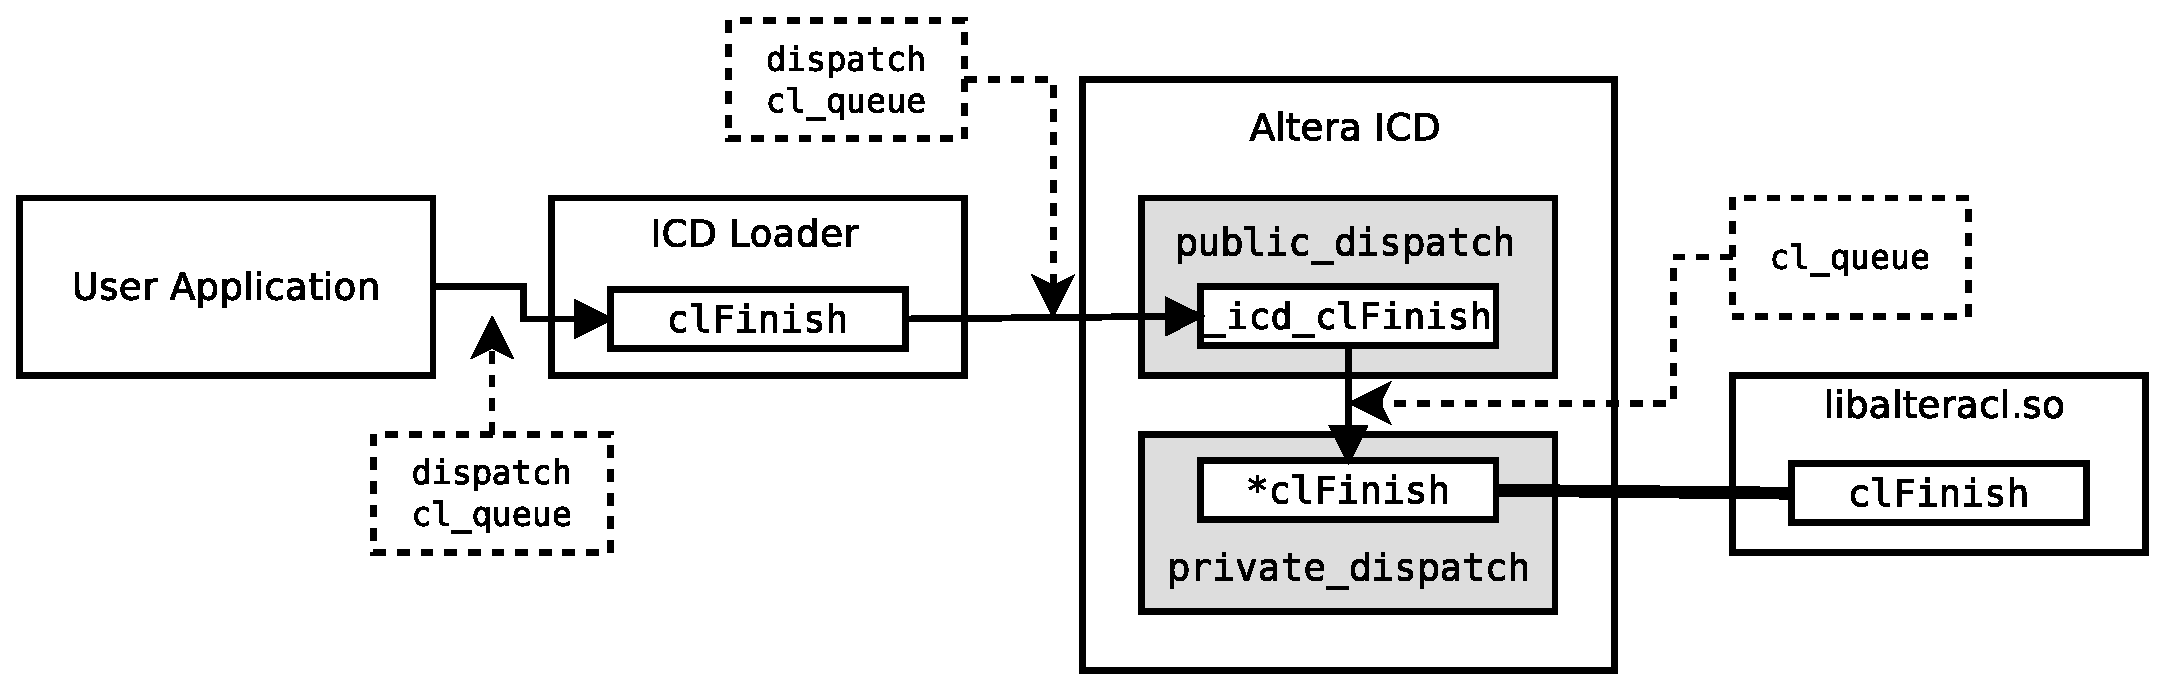
\includegraphics[width=1.1\textwidth]{images/icd3.eps}}
\caption{Call graph for the function \texttt{clFinish}.
The application calls the ICD loader function, which forwards the call to the wrapper function in the vendor ICD stored in the dispatch struct.
The wrapper function then calls the real OpenCL function.
The dashed boxes illustrate the contents of the arguments.}
\label{fig:icd2}
\end{figure}




%actual implementation
%The ICD loader opens the individual ICD libraries with the \texttt{dlopen} function \emph{without} the \texttt{RTLD\_DEEPBIND} flag \cite{icdloadersrc}.

The Altera ICD cannot be linked to the main library \texttt{libalteracl.so} which defines the actual OpenCL functions during compile time. This would again result in symbol conflicts, this time with the ICD Loader.
Instead, it must be loaded with \texttt{dlopen} during the run time.
\texttt{libalteracl.so} depends on \texttt{libelf.so}, \texttt{libalterammdpcie.so} and \texttt{libalterahalmmd.so}, which means these libraries have to be loaded beforehand with the \texttt{RTLD\_GLOBAL} flag.
This flag allows subsequently loaded libraries to use the symbols defined in the library to be loaded \cite{dlopen}.
While the \texttt{libelf.so} can be loaded without problems, the other two libraries in turn depend on \texttt{libalteracl.so} itself, creating a circular dependency.
A solution to this problem is to open \texttt{libalteracl.so} first with the \texttt{RTLD\_LAZY} flag and afterwards the other libraries with the opposite flag \texttt{RTLD\_NOW}.
With \texttt{RTLD\_LAZY}, a lazy binding is performed, that means the symbols are only resolved when needed, whereas \texttt{RTLD\_NOW} resolves all symbols before \texttt{dlopen} returns \cite{dlopen}.


Moreover to avoid conflicts with already loaded OpenCL symbols (defined by the ICD loader itself), the flag \texttt{RTLD\_DEEPBIND} is required.
This flag specifies that the library to be loaded should use its own symbols in preference to already loaded global symbols with the same name \cite{dlopen}.
The correct sequence of \texttt{dlopen} operations and flags is shown in listing \ref{listing:dlopen}.

\begin{lstlisting}[label=listing:dlopen, caption=Dynamically loading Altera OpenCL libraries, morekeywords={}]
dlopen( "libelf.so", RTLD_NOW | RTLD_GLOBAL | RTLD_DEEPBIND );
dlopen( "libalteracl.so", RTLD_LAZY | RTLD_GLOBAL | RTLD_DEEPBIND );
dlopen( "libalterammdpcie.so", RTLD_NOW | RTLD_GLOBAL | RTLD_DEEPBIND );
dlopen( "libalterahalmmd.so", RTLD_NOW | RTLD_GLOBAL | RTLD_DEEPBIND );
\end{lstlisting}


Loading the actual functions is accomplished with the \texttt{dlsym} function as in listing \ref{listing:dlsym}.
They will be stored in a second dispatch struct, only for use within the ICD.


\begin{lstlisting}[label=listing:dlsym, caption=Dynamically loading the original \texttt{clFinish} and filling in the dispatch, morekeywords={}]
private_dispatch.clFinish 
   = (KHRpfn_clFinish)dlsym(libalteracl_handle, "clFinish");
errmsg=dlerror();
if(errmsg!=NULL){return(-1);}
public_dispatch.clFinish=&_icd_clFinish;
\end{lstlisting}





The OpenCL specification defines more than 100 functions, most of them are very rarely used.
Therefore only the following most common OpenCL functions have been wrapped for this thesis:
\begin{center}
\begin{tabular}{ l  l  l}
	\texttt{clGetPlatformIDs} & \texttt{clGetPlatformInfo} & \texttt{clGetDeviceIDs}\\
	\texttt{clGetDeviceInfo}& \texttt{clCreateCommandQueue} & \texttt{clCreateContext} \\
	\texttt{clCreateBuffer} &   \texttt{clCreateProgramWithBinary} & \texttt{clBuildProgram}\\
	\texttt{clCreateKernel} & \texttt{clEnqueueNDRangeKernel} &   \texttt{clSetKernelArg}\\
	\texttt{clEnqueueReadBuffer} &   \texttt{clEnqueueWriteBuffer} & \texttt{clFinish}\\
\end{tabular}
\end{center}

Trying to call a function not in this list will result in a segmentation fault.
Moreover, none of the \texttt{clEnqueue*} functions listed above support OpenCL \emph{events}.
Events can be sometimes useful for asynchronous operations, i.e. those that do not block.
To support events, a complex memory management system that tracks the lifetime of the event objects is required.%, which goes beyond the scope of this thesis.


Though incomplete, this set of functions allows a fully functional OpenCL application to be built and used together with implementations from other vendors within the same process.
Additional functions can be added, as described above.

